% Created 2023-01-06 Παρ 17:28
% Intended LaTeX compiler: pdflatex
\documentclass[11pt]{article}
\usepackage[utf8]{inputenc}
\usepackage[T1]{fontenc}
\usepackage{graphicx}
\usepackage{longtable}
\usepackage{wrapfig}
\usepackage{rotating}
\usepackage[normalem]{ulem}
\usepackage{amsmath}
\usepackage{amssymb}
\usepackage{capt-of}
\usepackage{hyperref}
\usepackage{booktabs}
\usepackage{import}
\usepackage[LGR, T1]{fontenc}
\usepackage[greek, english]{babel}
\usepackage{alphabeta}
\usepackage{esint}
\usepackage{mathtools}
\usepackage{esdiff}
\usepackage{makeidx}
\usepackage{glossaries}
\usepackage{newfloat}
\usepackage{chemfig}
\usepackage{svg}
\usepackage[a4paper, margin=3cm]{geometry}
\author{Βιδιάνος Γιαννίτσης, Διονύσης Γιαννάτος, Αριστοτέλης Αργυρόπουλος \\ Θεοφανώ-Αντωνία Πόταρη, Στυλιανή Σταύρου, Έλλη Πούτα}
\date{\today}
\title{Ολοκληρωμένη Προσομοίωση Μετατροπής Πυρηνόξυλου σε Γλυκερόλη και Κυκλοπεντανόνη}
\hypersetup{
 pdfauthor={Βιδιάνος Γιαννίτσης, Διονύσης Γιαννάτος, Αριστοτέλης Αργυρόπουλος \\ Θεοφανώ-Αντωνία Πόταρη, Στυλιανή Σταύρου, Έλλη Πούτα},
 pdftitle={Ολοκληρωμένη Προσομοίωση Μετατροπής Πυρηνόξυλου σε Γλυκερόλη και Κυκλοπεντανόνη},
 pdfkeywords={},
 pdfsubject={},
 pdfcreator={Emacs 28.2 (Org mode 9.5.5)}, 
 pdflang={English}}
\makeatletter
\newcommand{\citeprocitem}[2]{\hyper@linkstart{cite}{citeproc_bib_item_#1}#2\hyper@linkend}
\makeatother

\usepackage[notquote]{hanging}
\begin{document}

\maketitle
\tableofcontents

\renewcommand{\abstractname}{Περίληψη}
\renewcommand{\tablename}{Πίνακας}
\renewcommand{\figurename}{Σχήμα}
\pagebreak
\section{Προσομοίωση των στερεών στο Aspen}
\label{sec:org89ec3e7}
Στην διεργασία που μελετήσαμε υπάρχουν 4 βασικά στερεά τα οποία δεν υπάρχουν στην βάση δεδομένων του Aspen. Το πρώτο είναι η πρώτη ύλη μας, το πυρηνόξυλο. Αυτό ορίστηκε ως nonconventional component και βρέθηκαν βιβλιογραφικά το proximate και ultimate analysis του. Επίσης, βρέθηκε η σύσταση του σε κυτταρίνη, ημικυτταρίνη και λιγνίνη και τα yields του σε steam explosion. \textsuperscript{\citeprocitem{1}{1}–\citeprocitem{5}{5}} . Από τα άρθρα αυτά βρέθηκε επίσης η θερμογόνος δύναμη της παραγόμενης λιγνίνης και η μετατροπή στην ενζυμική υδρόλυση της κυτταρίνης.

Μετά την προκατεργασία του πυρηνόξυλου, διαχωρίζεται στα κλάσματα του, κυτταρίνη, ημικυτταρίνη και λιγνίνη. Το ημικυτταρινικό κλάσμα είναι αυτό που είναι υδατοδιαλυτό και αυτουδρολύεται για αυτό δεν βρίσκουμε ημικυτταρίνη στην έξοδο αλλά τα συστατικά της. Άρα, τα δύο στερεά που πρέπει να προσομοιωθούν είναι η κυτταρίνη και η λιγνίνη. Για αυτά, ακολουθήθηκε η μεθοδολογία \textsuperscript{\citeprocitem{6}{6}} η οποία αναφέρει συγκεκριμένα την κυτταρίνη και την λιγνίνη. Η προσομοίωση αυτών στο Aspen αναφέρεται και πιό λεπτομερώς \href{https://github.com/Vidianos-Giannitsis/Process-Design/blob/master/lignin\_cellulose\_conventionals.org}{εδώ} .

Τέλος, πρέπει να προσομοιωθεί και η βιομάζα του μικροοργανισμού που κάνει την βιοαντίδραση μετατροπής της γλυκόζης σε γλυκερόλη. Αυτή έγινε με την ίδια λογική με αυτή των δύο παραπάνω.

\section{Χημικοί Αντιδραστήρες}
\label{sec:org4f13686}
Οι δύο βασικότεροι αντιδραστήρες της διεργασίας είναι οι αντιδραστήρες που παράγουν τα τελικά προιόντα μας.

\subsection{Παραγωγή Γλυκερόλης}
\label{sec:org332a527}
Ο πρώτος αντιδραστήρας είναι ο batch βιοαντιδραστήρας παραγωγής γλυκερόλης. Ο αντιδραστήρας είναι σε λειτουργία batch για να είναι σύμφωνος με την βιβλιογραφία \textsuperscript{\citeprocitem{7}{7},\citeprocitem{8}{8}}. Ακόμη, οι βιοαντιδραστήρες που λειτουργούν σε συνεχή λειτουργία, ιδιαίτερα για αντιδράσεις στις οποίες απαιτείται μεγάλος χρόνος παραμονής, όπως αυτή έχουν ένα μεγάλο μειονέκτημα. Υπάρχει η πιθανότητα επιμόλυνσης του αντιδραστήρα η οποία θα μειώσει την παραγωγικότητα του. Σε έναν batch βιοαντιδραστήρα αυτό θα επηρεάσει το πολύ ένα batch και μετά θα καθαριστεί. Στην περίπτωση της συνεχούς λειτουργίας όμως, απαιτείται ολικό shutdown της διεργασίας για να καθαριστεί, το οποίο μειώνει τον παραγωγικό χρόνο.

Ο αντιδραστήρας αυτός τροφοδοτείται με μία πηγή άνθρακα (την γλυκόζη), μία πηγή αζώτου (την ουρία) και οξυγόνο και έχει ως σκοπό την ανάπτυξη της αερόβιας καλλιέργειας του μικροοργανισμού Candida glycerinogenes. Μικρή ποσότητα βιομάζας εμβολιάζεται αρχικά στον αντιδραστήρα για να ξεκινήσει η αντίδραση. Η κινητική του μικροοργανισμού έχει μελετηθεί σύμφωνα με το αρχείο \href{https://github.com/Vidianos-Giannitsis/Process-Design/blob/master/c\_glycerinogenes\_rate\_expressions.org}{αυτό} και αποτελεί μία κινητική Monod προσαρμοσμένη σε βιβλιογραφικά δεδομένα \textsuperscript{\citeprocitem{7}{7}} ενώ η προσομοίωση του αντιδραστήρα στο Aspen επεξηγείται περισσότερο \href{https://github.com/Vidianos-Giannitsis/Process-Design/blob/master/Aspen/complete\_bioreactor.org}{εδώ}. Σημαντικό θέμα για την ανάλυση αυτή ήταν και η προσομοίωση του τύπου της βιομάζας, η οποία λόγω της αβεβαιότητας που είχαμε στο σύστημα ήταν αρκετά δύσκολη. Οι \textsuperscript{\citeprocitem{6}{6}} έχουν διατυπώσει μία μέθοδο για προσομοίωση συστατικών βιομάζας ως conventional solids στο Aspen στην οποία βασιστήκαμε. Το πως βρέθηκε ο τύπος της βιομάζας και τα απαιτούμενα χαρακτηριστικά του, φαίνεται \href{https://github.com/Vidianos-Giannitsis/Process-Design/blob/master/biomass\_modeling\_aspen.org}{εδώ}.

\subsection{Παραγωγή Κυκλοπεντανόνης}
\label{sec:orgad44900}
Η παραγωγή κυκλοπεντανόνης γίνεται με βάση την φουρφουράλη, ένα ενδιάμεσο προιόν που παράγετια από την ξυλόζη. Για αυτό απαιτείται ένας τρίτος αντιδραστήρας ο οποίος κάνει την αφυδάτωση της ξυλόζης σε φουρφουράλη ο οποίος θα αναφερθεί παρακάτω.

Για την παραγωγή κυκλοπεντανόνης, αρχικά το ρεύμα που είναι πλούσιο σε
φουρφουράλη τροφοδοτείται σε αντιδραστήρα συνεχούς ροής με προσθήκη
υδρογόνου H\textsubscript{2}. Ως προϊόντα της αντίδρασης λαμβάνεται η κυκλοπεντανόνη
και το νερό.

Στην προσομοίωση, για τον αντιδραστήρα, επιλέχτηκε το μοντέλο RCSTR, που
χρησιμοποιείται για την περιγραφή αντιδραστήρων συνεχούς ροής. Για τη
μοντελοποίηση του αντιδραστήρα, ορίστηκε η κινητική της αντίδρασης με το
μηχανισμό Powerlaw, που από την βιβλιογραφία η σταθερά της αντίδρασης
για 160\textsuperscript{ο}C είναι ίση με 0,0128 hr\textsuperscript{-1} με ενέργεια ενεργοποίησης 64,2
kJ/mol. Ο χρόνος που χρειάζεται η αντίδραση για να πραγματοποιηθεί σε
αυτές τις συνθήκες είναι 1 ώρα. Το θερμοδυναμικό μοντέλο που επιλέχθηκε
είναι το PRWS, λόγω της υψηλής θερμοκρασίας.

Η αντίδραση πραγματοποιείται ως εξής: Μετά τον θερμαντήρα, η φουρφουράλη
και το νερό, με την ίδια σύσταση που είχαν στην έξοδο του πρώτου
αντιδραστήρα (3960,56 kg/hr), εισέρχονται στον δεύτερο. Ταυτόχρονα,
εισέρχεται ποσότητα υδρογόνου με ρυθμό 159,54 kg/hr. Η στοιχειομετρία
της αντίδρασης είναι η εξής:

\[C_{5}H_{4}O_{2}  + 3H_{2}  \rightarrow  H_{2}O +  C_{5}H_{8}O \]

Αυτό έχει ως αποτέλεσμα η έξοδος του αντιδραστήρα να αποτελείται από τα
εξής προϊόντα και σύσταση:

\begin{figure}[htbp]
\centering
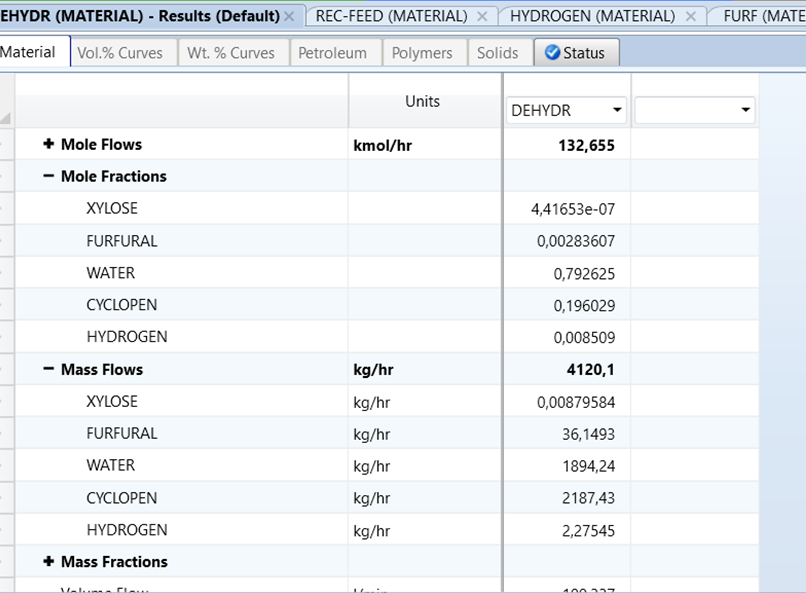
\includegraphics[width=.9\linewidth]{Χημικοί_Αντιδραστήρες/2023-01-06_16-54-14_screenshot.png}
\caption{Αποτελέσματα αντιδραστήρα Κυκλοπεντάνονης}
\end{figure}

\pagebreak
\begin{table}[htbp]
\caption{Πληροφορίες σχετικά με την αντίδραση παραγωγής κυκλοπεντανόνης από φουρφουράλη}
\centering
\begin{tabular}{ll}
Είδος Αντιδραστήρα & RCSTR\\
\hline
Θερμοδυναμικό Μοντέλο & PRWS\\
Ρεύματα: & Είσοδος: Φουρφουράλη, Υδρογόνο H\textsubscript{2}\\
 & Έξοδος: Κυκλοπεντανόνη και νερό H\textsubscript{2}O\\
\end{tabular}
\end{table}

\subsection{Παραγωγή Φουρφουράλης}
\label{sec:orga3a4107}
 Η αντίδραση που πραγματοποιείται είναι
η διάσπαση της ξυλόζης σε φουρφουράλη και νερό. Συνεπώς, στην είσοδο του
αντιδραστήρα ως τροφοδοσία θεωρείται το ημικυτταρινικό κλάσμα με κύριο
συστατικό την ξυλόζη, ενώ η έξοδος του αντιδραστήρα είναι πλούσια σε
φουρφουράλη και νερό.

Στην βιβλιογραφία \textsuperscript{\citeprocitem{9}{9}} χρησιμοποιούνται για την αντίδραση αυτή αντιδραστήρες συνεχούς έργου και υπάρχουν επαρκή
δεδομένα για την κινητική της αντίδρασης που μπορούν να χρησιμοποιηθούν
στην προσομοίωση, οπότε χρησιμοποιήθηκε το μοντέλο RCSTR. Η αντίδραση
περιγράφεται από τον μηχανισμό Powerlaw και από την βιβλιογραφία η
κινητική σταθερά της αντίδρασης (k) ισούται με 7,92*10\textsuperscript{20} και η
ενέργεια ενεργοποίησης είναι 167,9 kJ/mol. Ο αντιδραστήρας λειτουργεί σε
σταθερή πίεση 15.6 atm και θερμοκρασία 242\textsuperscript{o}C ώστε το ρεύμα εξόδου να
έχει την επιθυμητή σύσταση.

Για τις θερμοδυναμικές παραμέτρους χρησιμοποιήθηκε το θερμοδυναμικό
μοντέλο PRWS που βασίζεται στην καταστατική εξίσωση
Peng-Robinson-Wong-Sandler. Το μοντέλο αυτό μπορεί να χρησιμοποιηθεί σε
πολικά και μη πολικά συστατικά, για υψηλές θερμοκρασίες και πιέσεις
μέχρι 150 bar.

Στην είσοδο του αντιδραστήρα εισέρχεται ξυλόζη με ρυθμό 3960,56 kg/hr.
Στις συνθήκες που προαναφέρθηκαν, αυτή διασπάται σε νερό και φουρφουράλη
με την εξής στοιχειομετρία: \[ C_5H_{10}O_5 \rightarrow 3H_2O + C_5H_4O_2 \].

Αυτό έχει ως αποτέλεσμα στην έξοδο του αντιδραστήρα να εξέρχεται
φουρφουράλη με 2534,79 kg/hr και νερό με 1425,76 kg/hr.

\begin{table}[htbp]
\caption{Πληροφορίες σχετικά με την αντίδραση διάσπασης ξυλόζης σε φουρφουράλη και νερό}
\centering
\begin{tabular}{ll}
Είδος Αντιδραστήρα & RCSTR\\
\hline
Θερμοδυναμικό Μοντέλο & PRWS\\
Ρεύματα: & Είσοδος: Ξυλόζη\\
 & Έξοδος: Φουρφουράλη, Νερό\\
\end{tabular}
\end{table}

Για την προσομοίωση της ψύξης του μίγματος χρησιμοποιήθηκε το μοντέλο Heater. Ορίστηκε θερμοκρασία 160\textsuperscript{o}C και πίεση 15,8067 bar, για να
προσαρμόσει τις συνθήκες του ρεύματος φουρφουράλης πριν εισαχθεί στον
επόμενο αντιδραστήρα, χρησιμοποιώντας επίσης το θερμοδυναμικό μοντέλο
PRWS.

\subsection{Συμπληρωματικοί Αντιδραστήρες}
\label{sec:orgbd89ff0}
Για την προσομοίωση της ολοκληρωμένης διεργασίας που ζητήθηκε, απαιτούνται δύο ακόμη αντιδραστήρες. Ο πρώτος είναι ο αντιδραστήρας της ενζυμικής υδρόλυσης της κυτταρίνης σε γλυκόζη ώστε να μπορεί να χρησιμοποιηθεί ως το υπόστρωμα της βιοαντίδρασης. Για τον αντιδραστήρα αυτό έχει βρεθεί μία κινητική μελέτη \textsuperscript{\citeprocitem{10}{10}}, όμως, εν τέλει διαπιστώθηκε πως αυτή ήταν πολύ περίπλοκη και δεν υπήρχαν τα απαιτούμενα βιβλιογραφικά δεδομένα για να απλοποιηθεί. Καθώς ο αντιδραστήρας αυτός δεν είναι ένας από τους κεντρικούς αντιδραστήρες της διεργασιάς, δεν μελετήθηκε περαιτέρω το θέμα και η αντίδραση προσομοιώθηκε σε έναν αντιδραστήρα RStoic ως \(Cellulose + Water \rightarrow Glucose\) με την μετατροπή που βρέθηκε στην βιβλιογραφία \textsuperscript{\citeprocitem{1}{1}} .

Ο άλλος αντιδραστήρας είναι ο καυστήρας της λιγνίνης. Δεν αποτελεί κεντρικό αντιδραστήρα της διεργασίας, αλλά στην εκφώνηση του θέματος αναφέρθηκε πως η λιγνίνη του πυρηνόξυλου καίγεται, και μπορούμε να εκμεταλλευτούμε την θερμική ενέργεια αυτή για να θερμάνουμε άλλα ρεύματα της διεργασίας. Βρέθηκε η θερμογόνος δύναμη της λιγνίνης του πυρηνόξυλου \textsuperscript{\citeprocitem{5}{5}}, ένας ψευδομοριακός τύπος για να γραφεί η αντίδραση καύσης \textsuperscript{\citeprocitem{6}{6}} και η κινητική της καύσης αυτής \textsuperscript{\citeprocitem{11}{11}} και η προσομοίωση έγινε σε αντιδραστήρα CSTR. Περισσότερες λεπτομέρειες \href{https://github.com/Vidianos-Giannitsis/Process-Design/blob/master/Aspen/lignin\_combustion.org}{εδώ}.

Τα καυσαέρια αυτά βγαίνουν στους 1800 \(^oC\) περίπου και άρα είναι κατάλληλα για την παραγωγή ατμού υψηλής πίεσης που μπορεί να χρησιμοποιηθεί σε πολλά σημεία της εγκατάστασης για θέρμανση ρευμάτων.

\section{Βασικοί Διαχωρισμοί}
\label{sec:org79cc4b7}
Όπως και στους αντιδραστήρες, οι δύο βασικότεροι διαχωρισμοί είναι οι καθαρισμοί των δύο προιόντων. Επίσης σημαντικός διαχωρισμός όμως είναι η προκατεργασία της βιομάζας με την έκρηξη ατμού για την κλασματοποίηση της σε ημικυτταρινικό κλάσμα που θα χρησιμοποιηθεί για παραγωγή κυκλοπεντανόνης και στερεό κλάσμα (κυτταρίνη και λιγνίνη) και ο μετέπειτα διαχωρισμός κυτταρίνης και λιγνίνης ώστε η κυτταρίνη να υδρολυθεί σε γλυκόζη και να χρησιμοποιηθεί ως υπόστρωμα για την παραγωγή γλυκερόλης και η λιγνίνη να καεί.

\subsection{Καθαρισμός Γλυκερόλης}
\label{sec:orgadba994}
Το ρεύμα εξόδου από τον αντιδραστήρα αποτελείται από βιομάζα του μικροοργανισμού που αναπτύσσεται, τα κύρια προιόντα της αντίδρασης, γλυκερόλη, διοξείδιο του άνθρακα και νερό, τα παραπροιόντα της αντίδρασης, οξικό οξύ και αιθανόλη και ότι αντιδρώντα έχουν περισσέψει, κυρίως οξυγόνο και ουρία επειδή η γλυκόζη είναι το περιοριστικό υπόστρωμα της αντίδρασης.

Τα περισσότερα εκ'αυτών είναι αέρια ή πτητικά υγρά, με εξαίρεση της γλυκερόλης που έχει σημείο βρασμού 290 \(^oC\), άρα, με ένα flash μπορεί να γίνει ένας καλός πρώτος διαχωρισμός των συστατικών. Το flash αυτό πρέπει να γίνει σε θερμοκρασία όπου όλα τα υπόλοιπα συστατικά είναι σε μεγάλο βαθμό στην αέρια φάση. Επιλέχθηκε η θερμοκρασία των 140 \(^oC\), επειδή σε χαμηλότερες θερμοκρασίες από αυτήν δεν γινόταν καλός πρώτος διαχωρισμός, με αποτέλεσμα ο τελικός καθαρισμός να ήταν πολύ ενεργοβόρος και κοστοβόρος, ενώ σε υψηλότερες θερμοκρασίες άρχιζε να εξατμίζεται πολύ σημαντικότερη ποσότητα γλυκερόλης.

Μετά το flash, το υγρό κλάσμα το οποίο είναι γλυκερόλη, νερό που δεν εξατμίστηκε καθώς η αρχική του ποσότητα ήταν πολύ μεγάλη και βιομάζα, οδηγήθηκε σε ένα decanter στο οποίο διαχωρίστηκε η στερεή βιομάζα από το υγρό μίγμα. Τέλος, το μίγμα γλυκερόλης - νερού οδηγήθηκε σε μία αποστακτική στήλη με σκοπό τον καθαρισμό της γλυκερόλης και ανάκτηση γλυκερόλης με \(99.9 \%\) καθαρότητα.

Η στήλη αυτή, προσομοιώθηκε ως Radfrac στήλη με 6 βαθμίδες, λόγο αναρροής 0.175 mol και λόγο αποστάγματος προς τροφοδοσία 0.366 mol, σε θερμοκρασία και πίεση ίδιες με αυτές του flash (140 \(^oC\), 1 bar) η οποία καταφέρνει να εξατμίσει όλο το νερό με αποτέλεσμα να ανακτάται το \(90 \%\) της αρχικής γλυκερόλης με καθαρότητα 0.999.

Για την θέρμανση των προιόντων του αντιδραστήρα για να οδηγηθούν στο flash χρησιμοποιήθηκαν αποκλειστικά τα προιόντα της διεργασίας. Αρχικά, ψύχθηκε το ρεύμα της καθαρής γλυκερόλης μέχρι θερμοκρασία δωματίου για να αποθηκευτεί σε αυτήν και για το υπόλοιπο θερμικό φορτίο χρησιμοποιήθηκε το μίγμα του νερού της αποστακτικής στήλης μαζί με τους ατμούς του flash. Για να είναι εφικτή η μεταφορά θερμότητας μεταξύ των δύο ρευμάτων στην θερμοκρασία που θέλουμε, πρέπει τα αέρια αυτά να μπούν σε έναν συμπιεστή που αυξάνει την πίεση τους κάτα 1 bar ώστε να έχουν το θερμικό περιεχόμενο που απαιτείται για την θέρμανση αυτή. Περισσότερες λεπτομέρειες για την διάταξη των εναλλακτών αυτή υπάρχει \href{https://github.com/Vidianos-Giannitsis/Process-Design/blob/master/Aspen/heat\_exchange.org}{εδώ} . 

\subsection{Καθαρισμός Κυκλοπεντανόνης}
\label{sec:orgd4d343d}
Όπως διαπιστώθηκε από τον αντιδραστήρα, το ρεύμα που βγαίνει από τον τελικό αντιδραστήρα δεν είναι καθαρή κυκλοπεντανόνη. Πρέπει να γίνουν μερικές διεργασίες διαχωρισμών για να καθαριστεί.

\subsubsection{Διαχωρισμός Υδρογόνου}
\label{sec:org45e75eb}
Το ρεύμα εξόδου από τον δεύτερο αντιδραστήρα κατευθύνεται προς έναν
διαχωριστήρα, με σκοπό την αφαίρεση και ανακύκλωση εναπομείναντος
υδρογόνου, το οποίο βρίσκεται στην αέρια φάση.

Στο Aspen χρησιμοποιήθηκε Component Separator με το θερμοδυναμικό
μοντέλο Peng - Robinson με κανόνες ανάμιξης Wong -Sandler (PRWS) για
την πρόβλεψη των θερμοδυναμικών ιδιοτήτων του συστήματος. Για αυτόν
λοιπόν τον separator η πίεση είναι στα 40 bar, ίδιο με την πίεση εξόδου
από τον αντιδραστήρα κυκλοπεντανόνης, και το μίγμα μέσα σε αυτόν είναι
διφασικό (υγρό-ατμός).

Μέσω την χρήση του διαχωριστή, το μίγμα που προκύπτει από τον
αντιδραστήρα διαχωρίζεται σε δύο ρεύματα: Το ένα ρεύμα περιέχει
εξολοκλήρου υδρογόνο, το οποίο ανακυκλώνεται στον αντιδραστήρα της
κυκλοπεντανόνης, ενώ το άλλο ρεύμα που περιέχει την κυκλοπεντανόνη, την
φουρφουράλη και το νερό προχωράει στην αποστακτική στήλη για περεταίρω
επεξεργασία.

\subsubsection{Αποστακτική Στήλη Ανάκτησης Καθαρής Κυκλοπεντάνονης}
\label{sec:orgb895cf7}
Έπειτα, το ρεύμα που περιέχει κυκλοπεντανόνη ψύχεται σε εναλλάκτη
θερμότητας σε θερμοκρασία 160 \^{}\{ο\} C και πίεση 20 bar. Το θερμοδυναμικό
μοντέλο για τον εναλλάκτη είναι η Peng -- Robinson (PRWS). Στο Aspen ως
εναλλάκτης θερμότητας εφαρμόστηκε Heater.

Μετά τη ψύξη του, το ρεύμα εισέρχεται σε μια αποστακτική στήλη με σκοπό
τον διαχωρισμό της κυκλοπεντανόνης από το νερό. Αρχικά έγινε χρήση του
Azeotrope Finder για την εύρεση αζεότροπων, αλλά διαπιστώθηκε πως σε
πίεση 16 bar δεν υπάρχουν αζεότροπα. Εφόσον η πίεση του μίγματος είναι
40 bar από τον αντιδραστήρα υδρογόνωσης, επιλέχθηκε να γίνει απόσταξη σε
πίεση 16 bar.

Λόγω της έλλειψης αζεότροπων, στο Aspen έγινε χρήση της απλοποιημένης
στήλης DSTWU. Η στήλη περιέχει 55 βαθμίδες απόσταξης και ως προϊόν
κορυφής ανακτάται το νερό κατά \(99.9 \%\). Στο προϊόν κορυφής επιλέγεται η
κυκλοπεντανόνη να ανακτάται σε ποσοστό \(7.2 \%\), εφόσον μικρότερα ποσοστά
οδηγούν σε υπερβολικά μεγάλο αριθμό βαθμίδων και λόγων αναρροής. Η πίεση
στον συμπυκνωτή όσο και στον αναβραστήρα είναι 16 bar, δηλαδή θεωρείται
πως δεν υφίσταται πτώση πίεσης μέσα στην στήλη.

Από τους υπολογισμούς του Aspen προκύπτει ελάχιστος λόγος αναρροής 0.96,
πραγματικός λόγος αναρροής 6.61, ελάχιστος αριθμός βαθμίδων 49.39, Λόγος
αποστάγματος προς τροφοδοσίας 0.813, και βαθμίδα τροφοδοσίας 31.86.

Ως αποτέλεσμα, το ρεύμα κορυφής έχει μαζική παροχή 2049.85 kg/hr με το
νερό να αποτελεί το \(92.3 \%\) της συνολικής μάζας, και το ρεύμα πυθμένα έχει
μαζική παροχή 2067.98 kg/hr και η κυκλοπεντανόνη αποτελεί το \(98.2 \%\) της
συνολικής μάζας. Στην παρακάτω εικόνα φαίνονται τα αποτελέσματα της
στήλης

\begin{figure}[htbp]
\centering
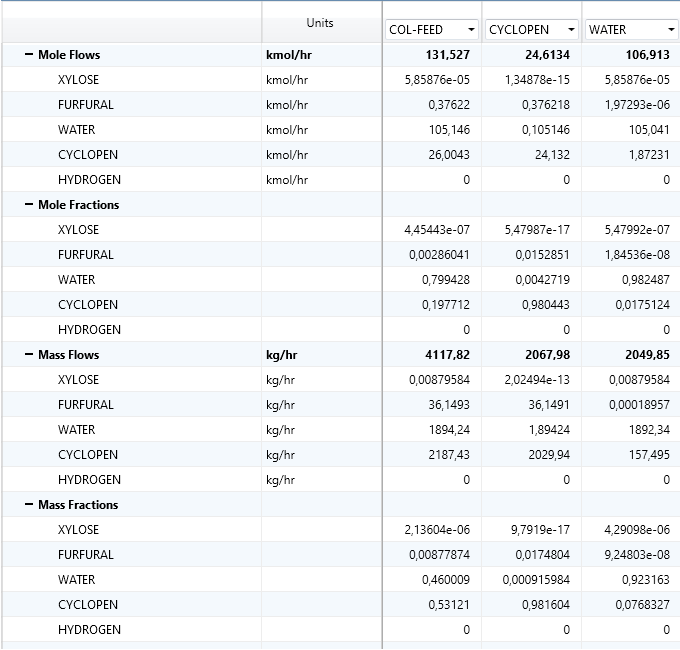
\includegraphics[width=.9\linewidth]{Βασικοί_Διαχωρισμοί/2023-01-06_17-08-54_screenshot.png}
\caption{Αποτελέσματα Αποστακτικής Στήλης}
\end{figure}

\begin{table}[htbp]
\caption{Πληροφορίες σχετικά με την αποστακτική στήλη}
\centering
\begin{tabular}{ll}
Είδος Στήλης & DSTWU\\
\hline
Θερμοδυναμικό Μοντέλο & PRWS\\
Ρεύματα: & Είσοδος: Κυκλοπεντανόνη, Φουρφουράλη, Νερό\\
Έξοδος: & Κορυφή: Νερό, Κυκλοπεντανόνη\\
 & Πυθμένας: Κυκλοπεντανόνη, Νερό, Φουρφουράλη\\
\end{tabular}
\end{table}


\subsection{Προκατεργασία Βιομάζας}
\label{sec:orgd8e10fe}
\subsubsection{Έκρηξη Ατμού}
\label{sec:org3cb8876}
Η διεργασία της έκρηξης ατμού είναι όπως προαναφέρθηκε μία σημαντική διεργασία για τον διαχωρισμό τον κλασμάτων της βιομάζας ώστε η ξυλόζη να χρησιμοποιηθεί για παραγωγή κυκλοπεντανόνης και η γλυκόζη για παραγωγή γλυκερόλης. Η διεργασία προσομοιώθηκε σε έναν αντιδραστήρα RYield καθώς είναι γνωστά από βιβλιογραφία \textsuperscript{\citeprocitem{1}{1},\citeprocitem{5}{5}} τα κλάσματα της βιομάζας αυτής. Οι υπολογισμοί αυτοί περιγράφονται \href{https://github.com/Vidianos-Giannitsis/Process-Design/blob/master/mass\_balances.org}{εδώ} και στο αντίστοιχο αρχείο στον φάκελο των υπολογισμών. Η λιγνίνη και η κυτταρίνη ορίστηκαν ως conventional solids όπως αναφέρθηκε παραπάνω ενώ η ημικυτταρίνη υδρολύθηκε κατά την διεργασία και άρα στο yield μπήκαν τα συστατικά της, τα οποία επίσης αναφέρονται στα παραπάνω άρθρα.

Για την διεργασία αυτή απαιτείται ατμός στα 26 bar και 232 \(^oC\) ο οποίος μπορεί να παραχθεί από την καύση περίπου του 1/8 της συνολικής λιγνίνης. Συγκεκριμένα, αυτή χρησιμοποιείται για την παραγωγή ατμού υψηλής πίεσης (40 bar) λίγο πάνω από το σημείο κορεσμού του (θεωρούμε πως αυτός είναι ο ατμός υψηλής πίεσης που διακινείται για θέρμανση/ψύξη ρευμάτων σε όλη την εγκατάσταση καθώς η τιμή αυτή είναι μία τυπική τιμή πίεσης για τέτοιο ατμό).  

\subsubsection{Διαχωρισμός των Στερεών}
\label{sec:orgedaa8c3}
Στην έξοδο του Steam Explosion υπάρχει μίγμα των δύο στερεών (κυτταρίνης και λιγνίνης) το οποίο πρέπει να διαχωριστεί. Με βάση την βιβλιογραφία \textsuperscript{\citeprocitem{1}{1}} η τυπική τεχνική για τον διαχωρισμό της κυτταρίνης από την λιγνίνη είναι η εκχύλιση με καυστικό νάτριο. Η λιγνίνη είναι διαλυτή σε αυτό και απομακρύνεται από την κυτταρίνη. Επειδή όμως το Aspen δεν μπορεί να προσομοιώσει εκχύλιση στερεού-υγρού και δεν έχει δεδομένα για την διαλυτότητα της λιγνίνης, αυτή η διεργασία προσομοιώθηκε με ένα απλό Separator στο οποίο ορίστηκε το βιβλιογραφικό yield. Η διεργασία αυτή βγάζει ένα ρεύμα κυτταρίνης με καθαρότητα 0.8, επειδή δεν μπορεί να ανακτηθεί όλη η λιγνίνη από το υδατικό διάλυμα καυστικού νατρίου.

Όμως, με βάση την βιβλιογραφία \textsuperscript{\citeprocitem{1}{1},\citeprocitem{5}{5}} η απόδοση της ενζυμικής υδρόλυσης πέφτει σημαντικά με παρουσία λιγνίνης καθώς αυτή δρα ανασχετικά στις κυτταρινάσες που χρησιμοποιούνται. Για αυτό προτείνεται μία διεργασία bleaching με NaClO\textsubscript{2} με την οποία μπορεί να απομακρυνθεί όλη η ποσότητα της λιγνίνης από το ρεύμα. Το διάλυμα που χρησιμοποιήθηκε είναι με βάση την βιβλιογραφία \textsuperscript{\citeprocitem{5}{5},\citeprocitem{12}{12}} . Για την καλή λειτουργία του, πρέπει να προθερμανθεί και στους 70 \(^oC\) το οποίο γίνεται με χρήση των ατμών στην έξοδο του steam explosion.

Έτσι, ανακτάται η καθαρή κυτταρίνη για να υδρολυθεί προς γλυκόζη. Περισσότερες λεπτομέρειες για τις προσομοιώσεις αυτές υπάρχουν \href{https://github.com/Vidianos-Giannitsis/Process-Design/blob/master/Aspen/lignin\_cellulose\_separation.org}{εδώ} .

\section{Στάδιο Ολοκληρωμένου Σχεδιασμού}
\label{sec:orgc17372e}
Οι προσομοιώσεις που έχουν γίνει είναι χωρισμένες σε 3 αρχεία. Ένα αρχείο που έχει όλη την προκατεργασία της βιομάζας, ξεκινόντας από το πυρηνόξυλο και φτάνοντας μέχρι την καθαρή γλυκόζη, λιγνίνη και ημικυτταρινικό κλάσμα ξυλόζης, το οποίο υπάρχει \href{https://github.com/Vidianos-Giannitsis/Process-Design/blob/master/Aspen/olive\_kernel\_to\_glucose\_complete.apwz}{εδώ} . Ένα αρχείο όπου έχει την βιοαντίδραση και τον καθαρισμό της γλυκερόλης ξεκινόντας με πρώτη ύλη την γλυκόζη, αναμεμιγμένη με τα άλλα θρεπτικά συστατικά και οξυγόνο, το οποίο υπάρχει \href{https://github.com/Vidianos-Giannitsis/Process-Design/blob/master/Aspen/glucose\_to\_glycerol\_complete.apwz}{εδώ}. Τέλος, ένα αρχείο με την διεργασία που ξεκινάει από την ξυλόζη, περνάει τους δύο αντιδραστήρες για παραγωγή φουρφουράλης και κυκλοπεντανόνης και τον καθαρισμό της κυκλοπεντανόνης, το οποίο υπάρχει \href{https://github.com/Vidianos-Giannitsis/Process-Design/blob/master/Aspen/xylose\_to\_cyclopentanone\_complete.apwz}{εδώ}.

Σε αυτά τα αρχεία έχουν αναγνωριστεί κάποια από τα βασικά ρεύματα ανακύκλωσης των διεργασιών και έχουν προσομοιωθεί. Επίσης, έχουν χρησιμοποιηθεί αρκετά ρεύματα εξόδου για προθέρμανση ή πρόψυξη άλλων ρευμάτων, για να έχουμε μία πρώτη εικόνα της ενεργειακής ολοκλήρωσης της διεργασίας. Υπάρχουν σημεία όπου αυτό δεν έχει γίνει ακόμη, αλλά έχει γίνει σε πολλά από τα βασικά στάδια της διεργασίας.

\section{Βιβλιογραφία}
\label{sec:org799a4b1}
\hypertarget{citeproc_bib_item_1}{(1) Fernandez-Bolanos, J.; Felizon, B.; Heredia, A.; Rodriguez, R.; Guillen, R.; Jimenez, A. Steam-Explosion of Olive Stones: Hemicellulose Solubilization and Enhancement of Enzymatic Hydrolysis of Cellulose. \textit{Bioresource technology} \textbf{2001}, \textit{79} (1), 53–61. \url{https://doi.org/10.1016/S0960-8524(01)00015-3}.}

\hypertarget{citeproc_bib_item_2}{(2) Domalski, E. S.; Jobe, T. L.; Milne, T. A. Thermodynamic Data for Biomass Conversion and Waste Incineration - NREL. \textbf{1987}, 326.}

\hypertarget{citeproc_bib_item_3}{(3) Gonzalez, J. F.; Gonzalez-Garcia, C. M.; Ramiro, A.; Gonzalez, J.; Sabio, E.; Ganan, J.; Rodrıguez, M. A. Combustion Optimisation of Biomass Residue Pellets for Domestic Heating with a Mural Boiler. \textit{Biomass and bioenergy} \textbf{2004}, \textit{27} (2), 145–154. \url{https://doi.org/10.1016/j.biombioe.2004.01.004}.}

\hypertarget{citeproc_bib_item_4}{(4) Koutsomitopoulou, A. F.; Bénézet, J. C.; Bergeret, A.; Papanicolaou, G. C. Preparation and Characterization of Olive Pit Powder as a Filler to PLA-matrix Bio-Composites. \textit{Powder technology} \textbf{2014}, \textit{255}, 10–16. \url{https://doi.org/10.1016/j.powtec.2013.10.047}.}

\hypertarget{citeproc_bib_item_5}{(5) Fernandez-Bolanos, J.; Felizon, B.; Heredia, A.; Guillen, R.; Jimenez, A. Characterization of the Lignin Obtained by Alkaline Delignification and of the Cellulose Residue from Steam-Exploded Olive Stones. \textit{Bioresource technology} \textbf{1999}, \textit{68} (2), 121–132. \url{https://doi.org/10.1016/S0960-8524(98)00134-5}.}

\hypertarget{citeproc_bib_item_6}{(6) Wooley, R. J.; Putsche, V. Development of an ASPEN PLUS Physical Property Database for Biofuels Components. \textbf{1996}, 36.}

\hypertarget{citeproc_bib_item_7}{(7) Jin, H.; Fang, H.; Zhuge, J. By-Product Formation by a Novel Glycerol-Producing Yeast, Candida Glycerinogenes, with Different O2 Supplies. \textit{Biotechnology letters} \textbf{2003}, \textit{25} (4), 311–314. \url{https://doi.org/10.1023/A:1022349401575}.}

\hypertarget{citeproc_bib_item_8}{(8) Zhuge, J.; Fang, H.-Y.; Wang, Z.-X.; Chen, D.-Z.; Jin, H.-R.; Gu, H.-L. Glycerol Production by a Novel Osmotolerant Yeast Candida Glycerinogenes. \textit{Applied microbiology and biotechnology} \textbf{2001}, \textit{55} (6), 686–692. \url{https://doi.org/10.1007/s002530100596}.}

\hypertarget{citeproc_bib_item_9}{(9) Yu, Z.; Li, Y.; Yao, Y.; Wang, Y.; Liu, Y.-Y.; Sun, Z.; Shi, C.; Wang, W.; Wang, A. Highly Selective Hydrogenative Ring-Rearrangement of Furfural to Cyclopentanone over a Bifunctional Ni3P/\$\gamma\$-Al2O3 Catalyst. \textit{Molecular catalysis} \textbf{2022}, \textit{522}, 112239. \url{https://doi.org/10.1016/j.mcat.2022.112239}.}

\hypertarget{citeproc_bib_item_10}{(10) Kadam, K. L.; Rydholm, E. C.; McMillan, J. D. Development and Validation of a Kinetic Model for Enzymatic Saccharification of Lignocellulosic Biomass. \textit{Biotechnology progress} \textbf{2004}, \textit{20} (3), 698–705. \url{https://doi.org/10.1021/bp034316x}.}

\hypertarget{citeproc_bib_item_11}{(11) Farrokh, N. T.; Suopajärvi, H.; Sulasalmi, P.; Fabritius, T. A Thermogravimetric Analysis of Lignin Char Combustion. \textit{Energy procedia} \textbf{2019}, \textit{158}, 1241–1248. \url{https://doi.org/10.1016/j.egypro.2019.01.413}.}

\hypertarget{citeproc_bib_item_12}{(12) Roy, A. K.; Bag, S. C.; Sardar, D.; Sen, S. K. Infrared Spectra of Jute Stick Bleached with Sodium Chlorite and Hydrogen Peroxide. \textit{Journal of applied polymer science} \textbf{1991}, \textit{43} (12), 2187–2192. \url{https://doi.org/10.1002/app.1991.070431205}.}
\end{document}